\chapter{Proceso}

Para la realización de este proyecto, se utilizará el proceso de software 'Prototipo'; proceso que permite generar iteraciones en las que se genera un prototipo en cada una de ellas,y que posteriormente será expuesto a pruebas y labores de mantenimiento para iniciar la siguiente iteración. Todo esto con la finalidad de obtener un producto final que cumpla con todos los requerimientos planteados para el buen funcionamiento.

\begin{figure}[h!]
	\centering
	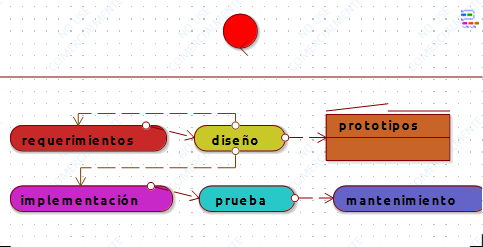
\includegraphics[width=0.7\linewidth]{proyecto/proceso/imgs/prototipo}
	\caption{Proceso Prototipo}
\end{figure}
\section{Implementación}

El proyecto será estructurado como un conjunto de módulos o componentes, los cuales serán organizados en una escala de dependencia, siendo desarrollados del más independiente al más dependiente. El proceso 'Prototipo' permitirá realizar una iteración por cada módulo propuesto, sin descartar hacer subiteraciones dentro de cada iteración; esto permitirá construir el prototipo final componente por componente. Es de aclarar que un componente no será agregado al prototipo final hasta que no esté totalmente depurado y funcional, tarea para la cual las iteraciones serán claves.


\subsection{Módulos}

\begin{figure}[h!]
	\centering
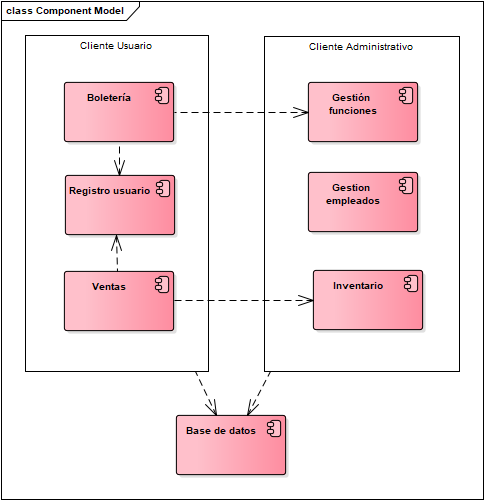
\includegraphics[width=0.7\linewidth]{proyecto/proceso/imgs/modulos}
	\caption{Módulos del sistema}
\end{figure}


\begin{itemize}
	\item{Cliente Usuario}
		\begin{enumerate}
			\item{\textbf{Registro usuario:} Módulo encargado de la inscripción, modificación y eliminación de usuarios dentro de la plataforma y de la gestión de las suscripciones especiales que existan dentro de la cadena de cines.}
			\item{\textbf{Boletería:} Módulo encargado de la visualización y selección de películas, selección de asientos y reservas y ventas de boletería.}
			\item{\textbf{Ventas:} Módulo encargado de visualizar el catálogo de comidas y accesorios y generar tickets de pago para las distintas ventas.}
		\end{enumerate}
	\item{Cliente Administrativo}
		\begin{enumerate}
			\item{\textbf{Gestión funciones:} Módulo encargado de agregar, eliminar y asignar funciones y salas a las distintas películas disponibles en el cinema, así como agregar próximos estrenos y eliminar películas de la cartelera.}
			\item{\textbf{Registro empleados:} Módulo encargado de llevar el registro de los empleados que trabajan en cada cinema, así como agregarlos o eliminarlos.}
			\item{\textbf{Inventario:} Módulo encargado de llevar control sobre el inventario de materia prima de confitería y maquinaria dentro de cada cinema.}
		\end{enumerate}
	\item{\textbf{Base de datos:} Módulo encargado de la insersión, actualización, modificación y almacenamiento de toda información que posteriormente utilizará el sistema}
\end{itemize}

\section{Diagrama de Gantt}
Se estimó el tiempo del proyecto en total 89 días, y bajo la premisa de que en promedio se dedicarán 10 días a cada uno de los modulos como máximo, teniendo como fecha de inicio el día 11 de abril y como fecha final el 8 de julio.
Teniendo en cuenta los módulos mostrados en la imagen 2.2 se llegó al acuerdo de que la forma más eficiente de sería desarrollarlos en el siguiente orden:
\begin{itemize}
	\item Módulo de bases de datos.
	\item Módulo de Gestión de empleados
	\item Módulo de Inventario.
	\item Módulo de Gestión de funciones.
	\item Módulo de Registro de Usuario.
	\item Módulo de ventas.
	\item Módulo de Boletería
\end{itemize}

En las imágenes 2.3 y 2.4 se muestran los tiempos dedicados para el desarrollo de cada uno de estos módules, mediante un diagrama de Gantt
\begin{figure}[h!]
	\centering
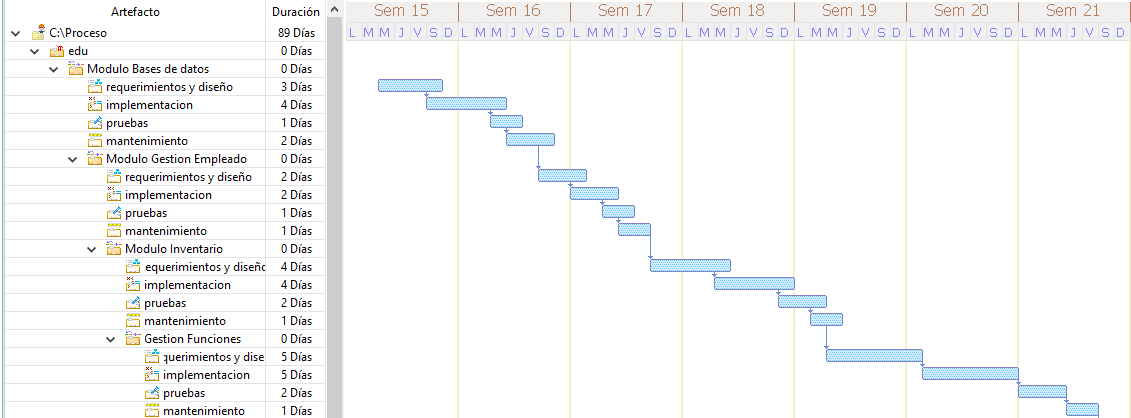
\includegraphics[width=1\linewidth]{proyecto/proceso/imgs/modulo1}
	\caption{Poyección del desarrollo (1)}
\end{figure}
\begin{figure}[h!]
	\centering
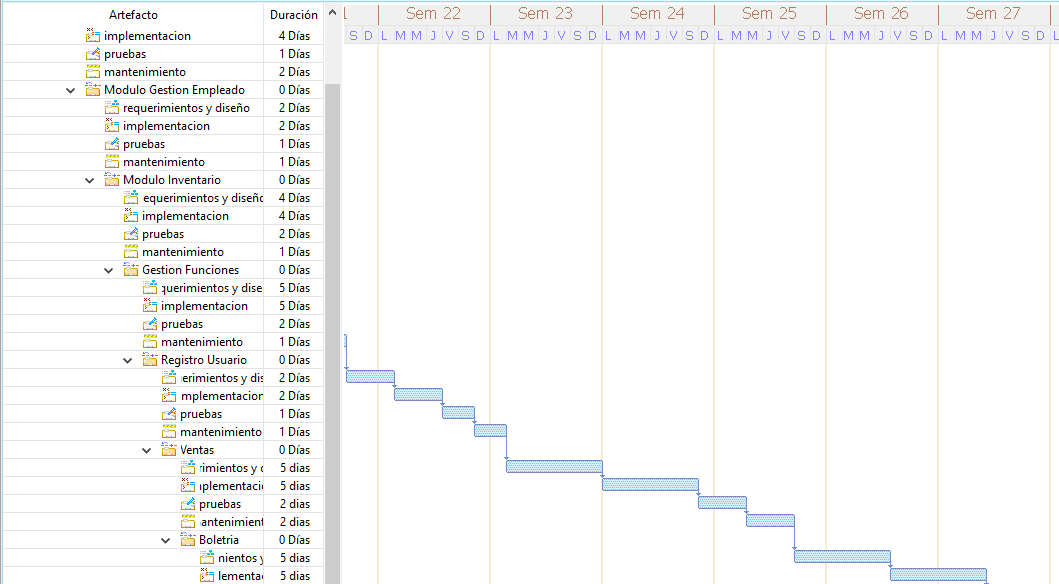
\includegraphics[width=0.9\linewidth]{proyecto/proceso/imgs/modulo2}
	\caption{Poyección del desarrollo (2)}
\end{figure}

\section{Metodología}
La metodología a usar durante la implementación de cada uno de los módulos del proyecto será la metodología 'SCRUM', la cual está estrechamente relacionada con el proceso de desarrollo 'Prototipo', ya que permite definir unos objetivos claros al inicio de cada iteración y posteriormente generar un entregable que permita evaluar lo hecho para iniciar una nueva iteración. Además de eso, esta metodología permite un desarrollo incremental, que permitirá corregir y agregar funcionalidades no previstas en un principio o que hayan sido mal concebidas en iteraciones anteriores.